\documentclass[10.5pt]{article}
\usepackage{amsmath}
\usepackage{graphicx}
\usepackage{hyperref}
\usepackage{mathtools}
\usepackage[latin1]{inputenc}
% \usepackage{exercise}
\usepackage{cancel}
\usepackage[margin=1.25cm]{geometry}
\usepackage{float}
\usepackage{multirow}
% \usepackage{wrapfig}
% \usepackage{amssymb}
% \usepackage{subfigure}
\setlength\parindent{0pt}

\title{Computational Neuroscience Project - Group 04}
\author{Giuseppe Leo, Francesco Negri}
\date{A.Y. 2022-2023}

\graphicspath{ {../images/} }

\begin{document}
\maketitle

\section*{Introduction}
The Leaky Integrate-and-Fire (LIF) and Integrate-and-Fire-or-Burst (IFB) models
are abstract neuronal models, aiming at reproducing the electrical physiological
behaviour of neurons.\\
These models describe the membrane potential \(V_{m}\) of the neuron:
whenever it overcomes the threshold voltage
\(V_{th}\), a spike is fired and the membrane potential goes back to \(V_{reset}\).\\
The LIF model is defined as follow:
\begin{align*}
    C_{m}\frac{dV_{m}}{dt} & =-I_{leak}+I_{stim}                           \\
                           & =-g_{leak}\bigl(V_{m}-E_{leak}\bigr)+I_{stim}
\end{align*}
On the other hand, the IFB neuron is modelled by these two differential equations:
\begin{align*}
    C_{m}\frac{dV_{m}}{dt}       & =-I_{leak}-I_{T}+I_{stim}                                                                                \\
                                 & =-g_{leak}\bigl(V_{m}-E_{leak}\bigr)-g_{T}h\bigl(V_{m}-E_{T}\bigr)\Theta\bigl(V_{m}-V_{h}\bigr)+I_{stim} \\
    \tau_{h}(V_{m})\frac{dh}{dt} & =-h+h_{\infty}(V_{m})
\end{align*}
where \(h_{\infty}(V_{m})=\Theta\bigl(V_{h}-V_{m}\bigr)\),
\(\tau_{h}(V_{m})=\tau_{h}^{-}\Theta\bigl(V_{m}-V_{h}\bigr)+\tau_{h}^{+}\Theta\bigl(V_{h}-V_{m}\bigr)\) and
\(\Theta\bigl(\,\cdot\,\bigr)\) is the Heaviside step function.\\
The two models are parametrized as shown in the table below:
\begin{table}[!h]
    \begin{center}
        \begin{tabular}{ |c||c|c|  }
            \hline
            \multicolumn{3}{|c|}{Models Parameters}                      \\
            \hline
            {}               & LIF neuron  & IFB neuron                  \\
            \hline
            \(S\)            & -           & \(3\cdot{10^{-4}}\;cm^{2}\) \\
            \(C_{m}\)        & \(100\;pF\) & \(2\;\mu{F}/cm^{2}\)        \\
            \(V_{0}\)        & \(-70\;mV\) & \(-58\;mV,\;\;-77\;mV\)     \\
            \(V_{reset}\)    & \(-70\;mV\) & \(-60\;mV\)                 \\
            \(V_{th}\)       & \(-50\;mV\) & \(-50\;mV\)                 \\
            \(V_{h}\)        & -           & \(-70\;mV\)                 \\
            \(V_{spike}\)    & \(20\;mV\)  & \(20\;mV\)                  \\
            \(g_{leak}\)     & \(10\;nS\)  & \(0.035\;mS/cm^{2}\)        \\
            \(E_{leak}\)     & \(-70\;mV\) & \(-75\;mV\)                 \\
            \(g_{T}\)        & -           & \(0.8\;mS/cm^{2}\)          \\
            \(E_{T}\)        & -           & \(120\;mV\)                 \\
            \(T_{ref}\)      & \(0\;s\)    & \(0\;s\)                    \\
            \(\tau_{h}^{+}\) & -           & \(100\;ms\)                 \\
            \(\tau_{h}^{-}\) & -           & \(20\;ms\)                  \\
            \hline
        \end{tabular}
        \caption{\label{table:parameters}The parameters used for the LIF and IFB neurons, respectively.}
    \end{center}
\end{table}

Note that in the following all the differential equations are solved by means of the Euler
method and the selected time step is \(\Delta{t}=0.1\;ms\).

\newpage

\section*{Question (a)}
The first two rows of Figure \ref{fig:Vm} show the trend
of the membrane potential \(V_{m}\) for the LIF and IFB models respectively in
the without noise condition.\\
The applied current \(I_{stim}\) in both models is a DC current with a step described as:
\begin{align*}
    I_{stim}(t) = I_0+I_1\cdot\Theta\bigl(t-t_{on}\bigr)
\end{align*}
where a constant value \(I_{0}\) is summed to a current \(I_{1}\) between the \(t_{on}=0.15\;s\)
and \(t_{off}=0.85\;s\) time instants. The total simulation duration is \(1\;s\).\\
We selected current values allowing to appreciate both sub- and supra-threshold behaviours.
In particular, for the LIF neuron we chose \(I_0=0\;pA\) and a current
\(I_1\in\{190,\dots{,250}\}\;pA\). On the other hand, the IFB model was excited by
a current described by \(I_0=230\;pA\) and \(I_1\in\{10,\dots{,250}\}\;pA\), compliant
with what is usually done in literature.\\

We can see in both cases - i.e., LIF and IFB models - that for small currents
the sub-threshold condition is observed: the membrane voltage \(V_{m}\) depolarizes, but
not enough to reach the threshold voltage \(V_{th}\), hence no spike is fired.
On the contrary, in the supra-threshold case the current must be larger, thus the neuron 
manages to overcome \(V_{th}\), eliciting spikes. 
Note that the number of action potentials fired in the same time window increases together with the 
amplitude of the stimulation current, both for LIF and IFB models.

\section*{Question (b)}
In order to experimentally infer the threshold voltage \(V_{th}^{*}\) it is
necessary to find the threshold current \(I_{th}\) from the gain function
depicted in Figure \ref{fig:gain},
which corresponds to the largest amount of input current not eliciting
spikes - i.e., exhibiting sub-threshold behaviour. After that,
such \(I_{th}\) is fed into the model as \(I_{stim}\) and the threshold voltage
is obtained as the maximum of \(V_{m}\), corresponding to the highest
depolarizing voltage before emitting a spike.\\
In both cases the obtained \(V_{th}^{*}\) is extremely close to the configured
model parameter \(V_{th}=-50\;mV\), available for either LIF and IFB models.

\section*{Question (c)}
Figure \ref{fig:gain} shows the gain function computed for the two models,
providing also a zoom (with an increase in the number of sampled points)
around the \(I_{th}\) current value, catching the transition between
sub-threshold and supra-threshold regimes.\\
The LIF neuron is assumed to belong to \textit{class II}, as a matter of fact 
it cannot fire at an arbitrarily low frequency, in particular the minimum
firing rate \(\nu(I_{stim})\simeq{15}\;Hz\).\\
Differently, the IFB neuron is considered to belong to \textit{class I}, as it is able to fire
even at very low frequencies (\(\nu(I_{stim})\simeq{2\;Hz}\)) for input currents slightly larger than \(I_{th}\).\\
In addition, it is important to point out that a difference exists in the behaviour of the
two neurons. As a matter of fact, both models have a regular spiking regime; however,
the IFB model allows to simulate bursting patterns as well, as displayed in Figure
\ref{fig:burst}. To switch between the two conditions, model parameters need to be
properly adjusted. The initial membrane potential \(V_{0}=V_{m}(0)\) is \(-58\;mV\) for tonic 
spiking and \(-77\;mV\) for the bursting activity. Moreover, the stimulation current
\(I_{stim}\) plays a curcial role as well. In particular, to have bursts, a larger
step of current is required with respect to the regular firing case.\\
Note that due to the absence of a refractory period (\(T_{ref}=0\;s\)) the gain function
for the two models increases almost linearly with the applied current, without reaching a plateau.

\section*{Question (d)}
A noisy stimulation current \(I_{stim}\) is obtained by adding a Gaussian noise with
mean \(\mu=0\) and standard deviation \(\sigma\) equal to \(1/100\) of the maximum value
of the input current. As seen in Figure \ref{fig:gain}, the first consequence observed by introducing noise
is that both
models display a slightly lower threshold current \(I_{th}\), which must be overcome
to elicit spikes. The LIF model minimum firing rate \(\nu(I_{stim})\) decreases from
about \(15\;Hz\) to approximately \(6\;Hz\). On the other hand, the IFB model minimum firing
rate \(\nu(I_{stim})\) is more or less halved, passing from \(2\;Hz\) to \(1\;Hz\).\\
Due to the decrease in the LIF model minimum firing rate, its behaviour
tends to be more similar to the one a \textit{class I} neuron.\\
Another significant difference with respect to case in which noise is not taken
into account is that here spikes are not fired at an extremely fixed frequency, though
they still keep a pretty regular pattern. This is due to the 
fluctuations in the amplitude of the stimulation current \(I_{stim}\) introduced by
the presence of noise, as illustrated in Figure \ref{fig:Vm}.

\begin{figure}
    \includegraphics[scale=0.065]{Vm}
    \centering
    \caption{Membrane potential \(V_{m}\) as a function of time \(t\) for several
    values of applied current \(I_{stim}\). A) LIF model without noisy stimulation current.
    B) IFB model in tonic firing pattern without noisy stimulation current. C) LIF model with
    noise in the input current. D) IFB model in tonic firing pattern with noise in the input current.}
    \label{fig:Vm}
\end{figure}

\begin{figure}
    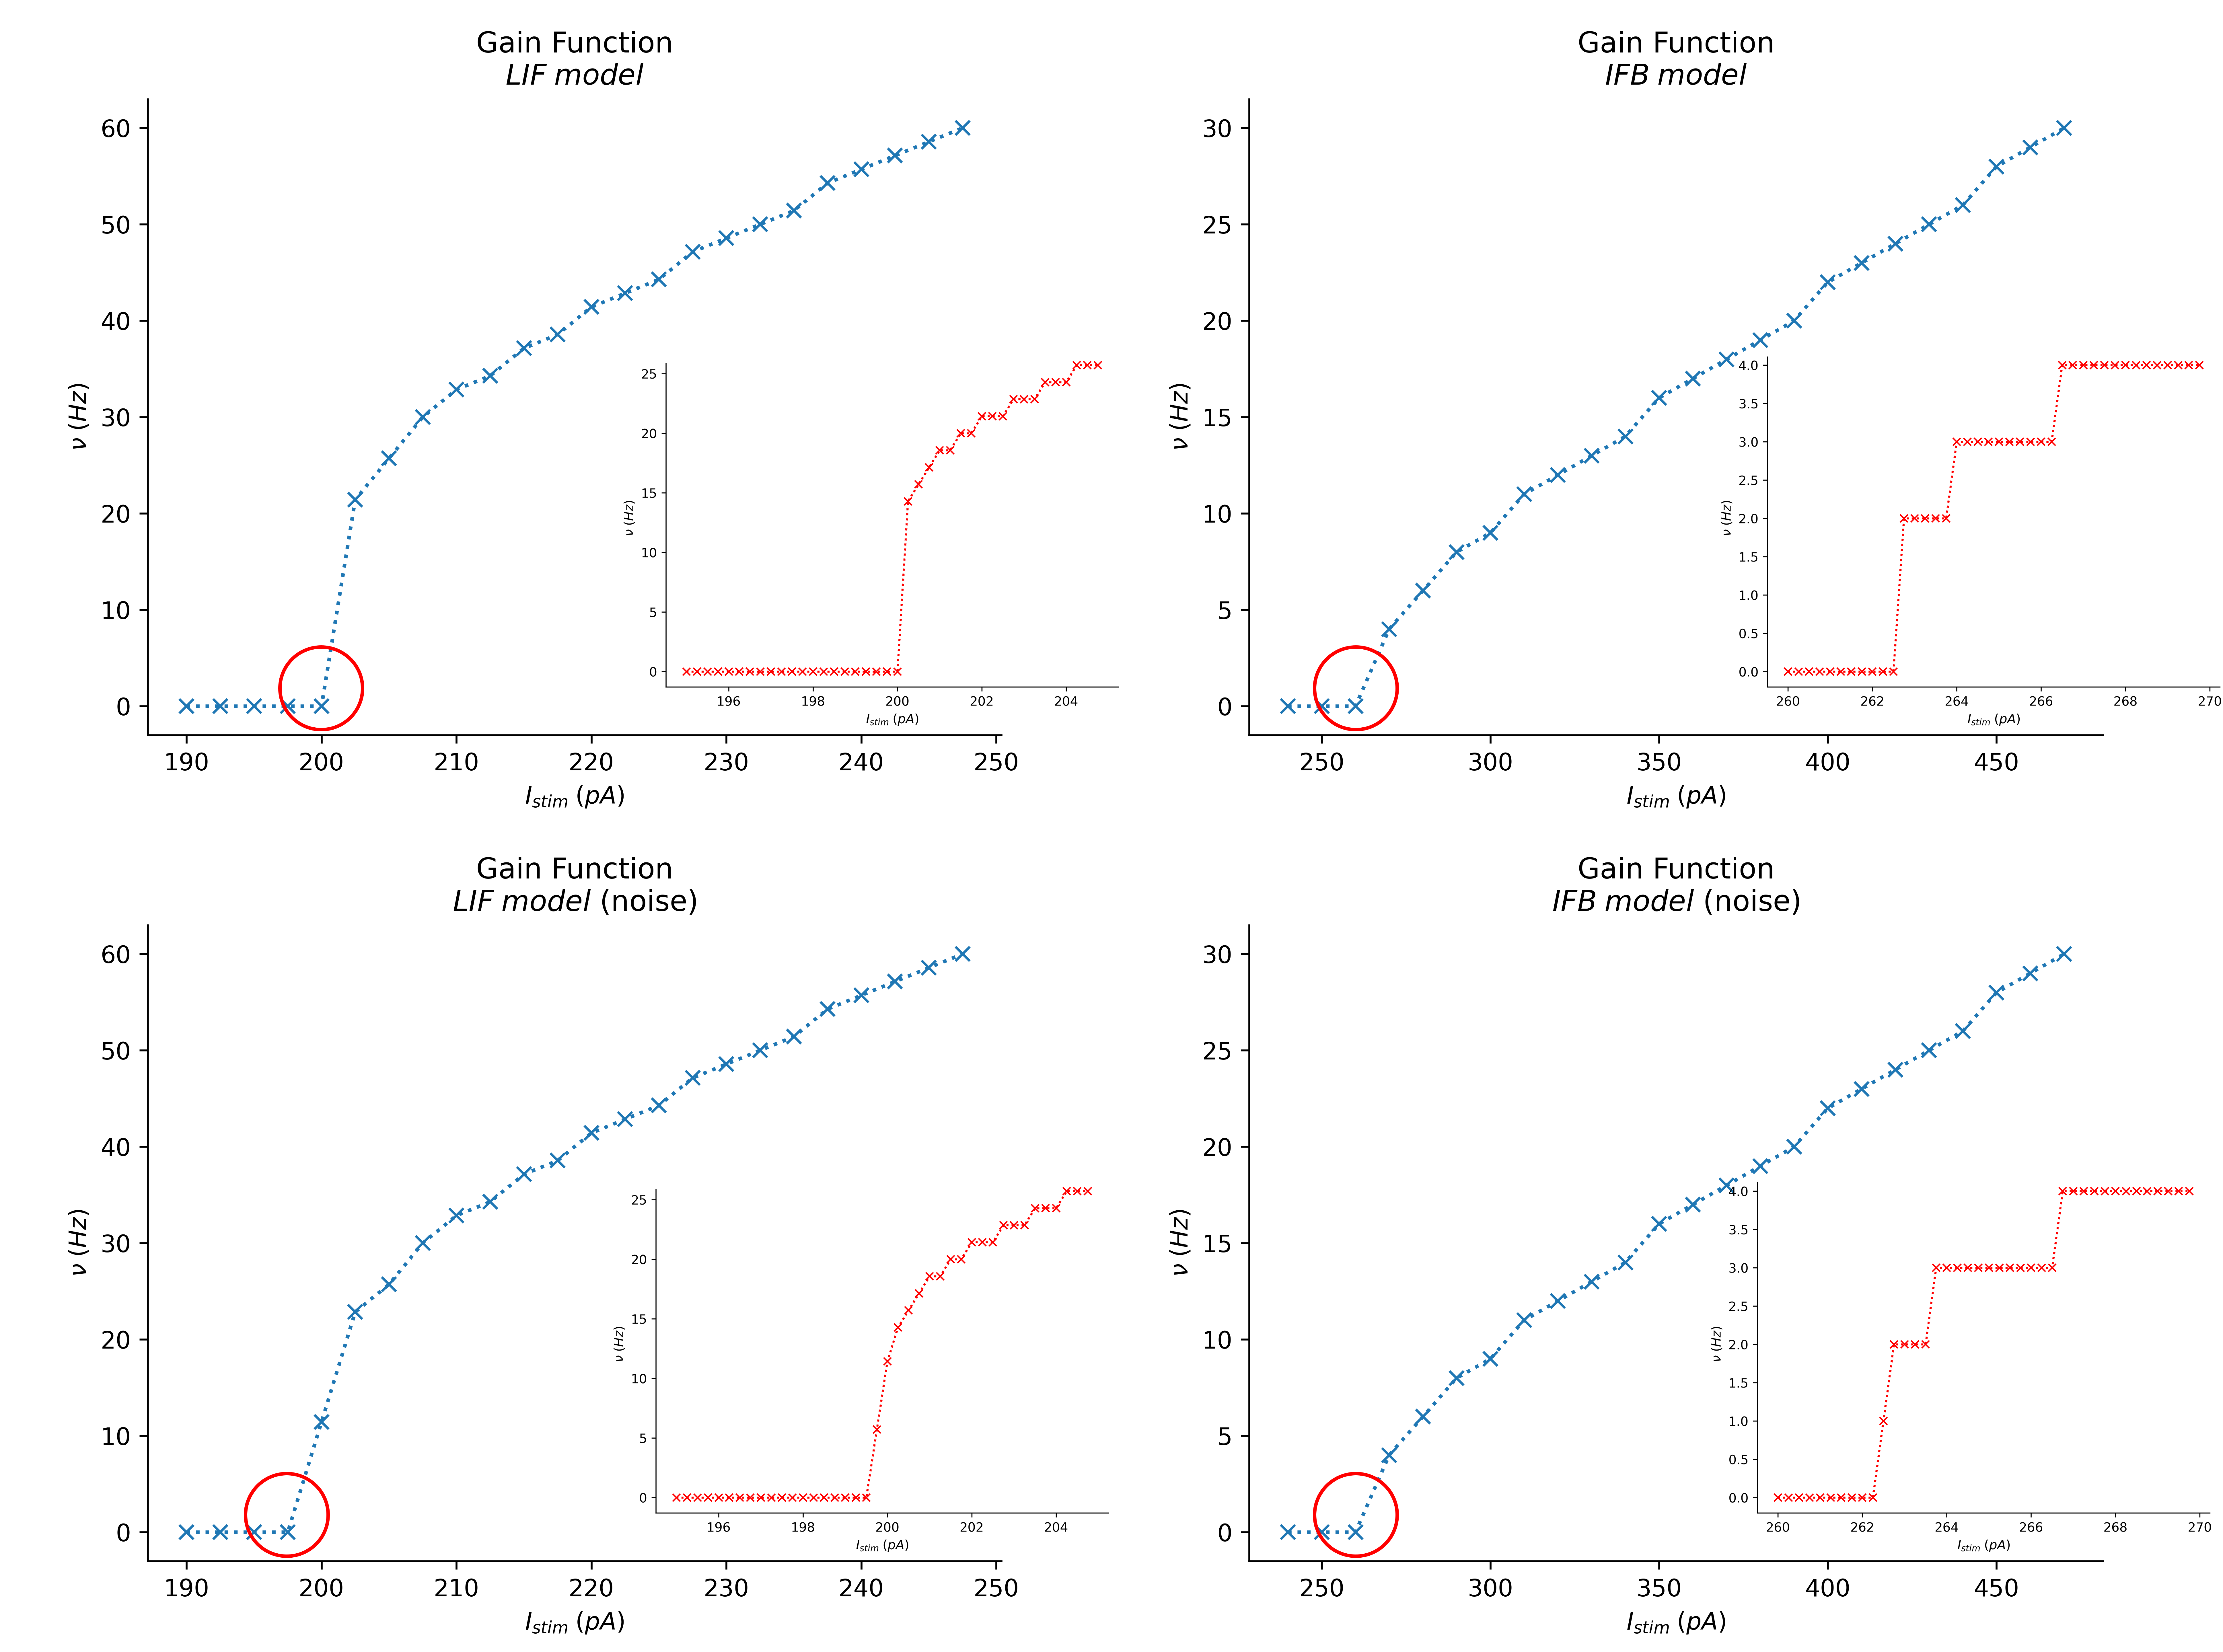
\includegraphics[scale=0.065]{gain}
    \centering
    \caption{Gain functions for all the models and
    conditions. The firing rate \(\nu\) is shown
    against the applied current \(I_{stim}\). Every plot
    includes a zoom (in red) around the \(I_{th}\) value,
    highlighting the transition area from
    sub-threshold to supra-threshold regime.
    A) LIF model without noisy stimulation current.
    B) IFB model in tonic firing pattern without noisy stimulation current. C) LIF model with
    noise in the input current. D) IFB model in tonic firing pattern with noise in the input current.}
    \label{fig:gain}
\end{figure}

\begin{figure}
    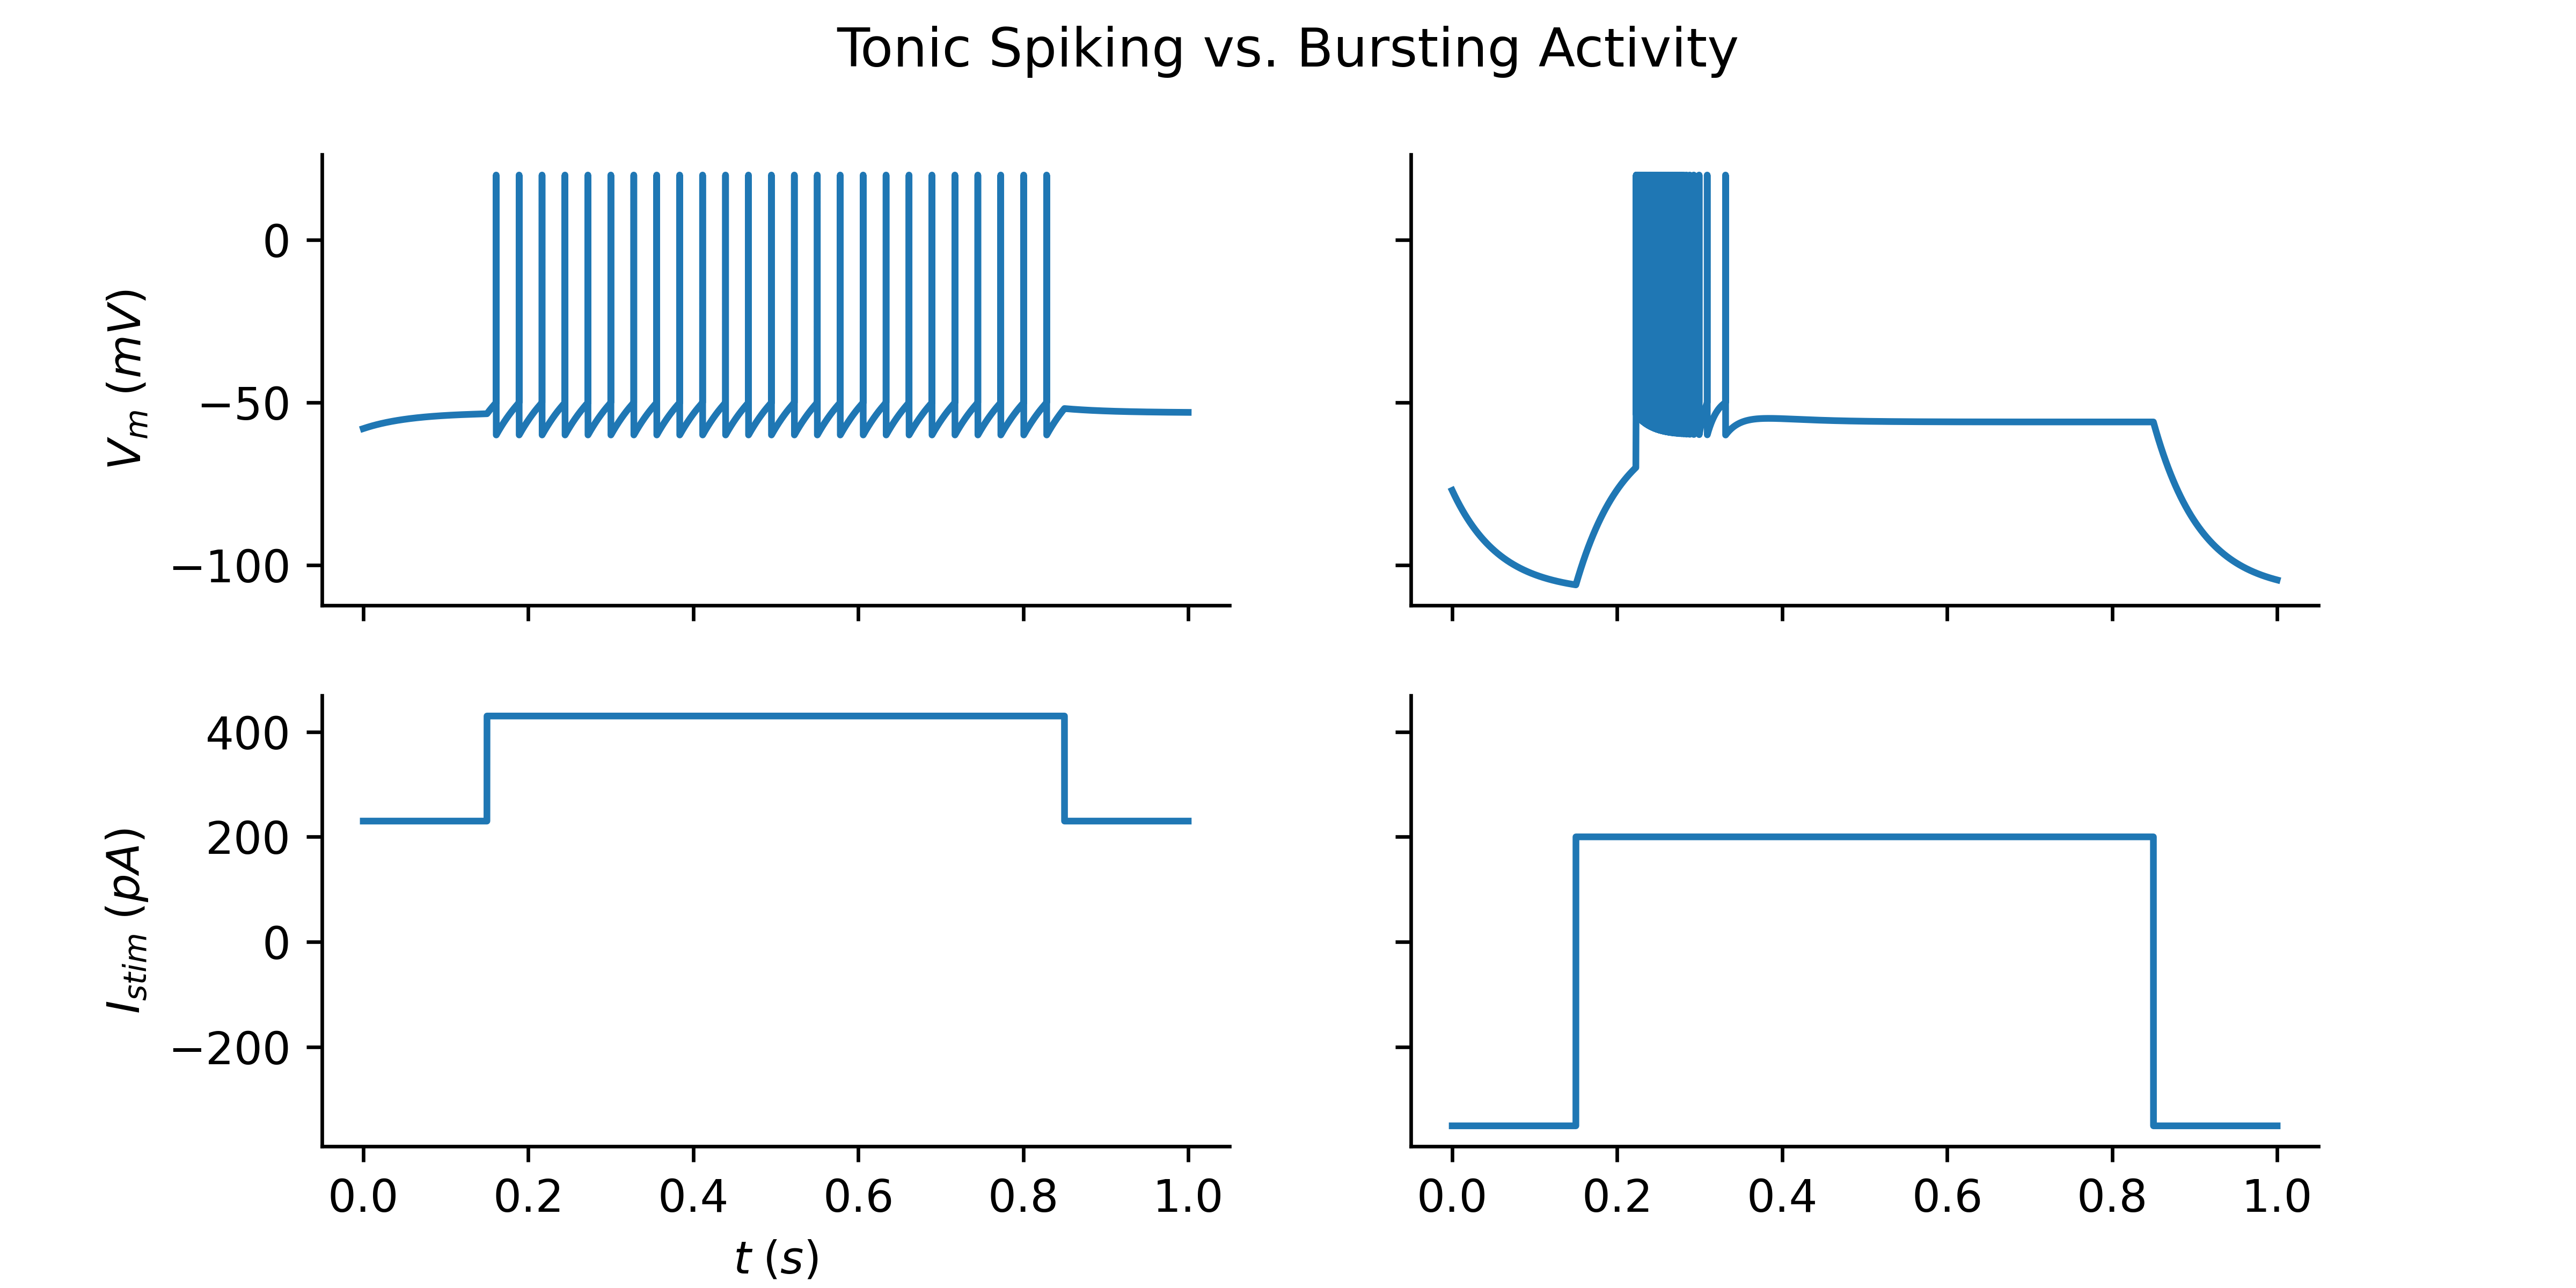
\includegraphics[scale=0.7]{IFB_tonic_bursting}
    \centering
    \caption{A comparison between the two behaviours
    of the IFB neuron: on the left the model is
    exhibiting tonic firing activity, while on the
    right it produces a burst. This is due to
    the difference in the model initial membrane voltage \(V_{0}\)
    and in the stimulation current \(I_{stim}\).}
    \label{fig:burst}
\end{figure}

\nocite{*}

\bibliographystyle{abbrv}
\bibliography{./citation}

\end{document}